\documentclass{article}

\usepackage[english]{babel}
\setlength\parindent{0pt} % Removes all indentation from paragraphs
%\usepackage{times} % Uncomment to use the Times New Roman font

\usepackage{color}
	\definecolor{darkred}{rgb}{0.55, 0.0, 0.0}
	\definecolor{keywords}{RGB}{255,0,90}
	\definecolor{comments}{RGB}{0,0,113}
	\definecolor{red}{RGB}{160,0,0}
	\definecolor{green}{RGB}{0,150,0}

\usepackage{amssymb,amsmath}
\usepackage{mathtools}

\usepackage{placeins}

\usepackage{wrapfig}
\usepackage{graphicx}
\usepackage{caption}
\usepackage{subcaption}

\usepackage{hyperref}

\usepackage{listings}
\lstset{language=Python, 
        basicstyle=\ttfamily\small, 
        keywordstyle=\color{keywords},
        commentstyle=\color{comments},
        stringstyle=\color{red},
        showstringspaces=false,
        identifierstyle=\color{green},
        title=\lstname}
%------------------------------------------------------------------------------%
%------------------------------------------------------------------------------%                                   
\title{Machine Learning \\ \bf{Exercise 4: Generative non-parametric classification:\\
								Naive Bayes and Density trees} } % Title
%------------------------------------------------------------------------------%                                   
% Document
%------------------------------------------------------------------------------%                                   

\begin{document}

\maketitle

\begin{center}
\begin{tabular}{l l}
Group: &  Sergej Kraft \\
       & Elias Roeger \\
       & Ekaterina Tikhoncheva \\ 
\end{tabular}
\end{center}

\tableofcontents

\section{Data set}

In this exercise we used the MNIST dataset, containing images of the handwritten digits. The size of the original images was to big for our purpose, so we used provided compressed version of the dataset, from which we picked up images with handwritten threes and eights.

For further dimension reduction of the feature space to the size of $2$ we used as corresponding function, we wrote for the exercise $2$: 

\lstinputlisting[language=Python]{dr.py}

\FloatBarrier

\section{Naive Bayes}

\subsection{Classification}

As we know from the theory the assumption of the naive Bayes Methode is, that all features are independent. That means:
$$p(y=k|x)=\frac{\prod_{j=1}^d p(x_j|y=k) p(y=k)}{\prod_{j=1}^d p(x_j)}$$

Our aim is therefore to learn for each class $k$ one dimension histograms $p(x_j|y=k)$ and prior $p(y=k)$.

The prior $p(y=k)$ is simply $N_k/N$, where $N_k$ is the number of elements in the training set from the class $k$ and $N$ is the size of the whole training set.

To learn the histograms we need an appropriate binning. We used the Freeman-Dice rule to compute the bin width. From the bin width we got the necessary number of bins pro dimension and class. If however the bin width was to small and thus the corresponding number of bin was too big, we forced the bin width to be $1/\sqrt[3]{N}$.

\begin{lstlisting}[language=Python]
# 			Choose proper bin size
def chooseBinSize(trainingx):
  
    n = trainingx.shape[0]
    d = trainingx.shape[1]
    
    # Choose bin width 
    dx = np.zeros(d, dtype = np.float128)
    L = np.zeros(d, dtype = np.int32)
    for j in range(0,d):
	# for each dimension apply Freeman-Diaconis Rule
        ind_sort =  np.argsort(trainingx[:,j]); # j-th feature dimension
        IQR = trainingx[ind_sort[3*n/4],j] - trainingx[ind_sort[n/4],j]        
        dx[j] = 2*IQR/np.power(n, 1/3.)        
        if dx[j]<0.01:
           dx[j] =  1/np.power(n, 1/3.)  
        m_j = (trainingx[ind_sort[n-1],j]-trainingx[ind_sort[0],j])/dx[j]   
        L[j] = np.ceil(m_j)
    # end for j
        
    return L, dx 
    # L number of bins pro dimension
    # dx bin width pro dimension
# end chooseBinSize
\end{lstlisting}

The learning function uses the given number of bins and bin width to calculate $1$-dimensional histograms pro class and dimension:

\begin{lstlisting}[language=Python]
##                          Naive Bayes Training
# determine priors  and likelihoods (for each feature and class individual 
# histogram <=> 4 histogramms  for two classes and two dimensions ) 
def naiveBayes_train_single_class(trainingx, trainingy, c, L, dx):
    # we consider one class c
    #    
    # trainingx is our training set    
    # trainingy are class labels for each element from trainingx
    # L number of bins pro dimension
    # dx bin width
        
    n = trainingx.shape[0]      # size of the training set
    d = trainingx.shape[1]      # size of the feature space
    
    # find  in training set all members of the class c
    xc = trainingx[trainingy==c, :]        # Class of digit c
    nc = xc.shape[0]

    ## Priors
    prior = nc/float(n)
    
    ## Likelihood p(x|y=c)
    
    histograms = [] 
  
    for j in range(0,d):
        
        histogram = np.zeros(L[j], dtype = np.float32)
        
        for i in range(0,nc):    
            l = np.ceil(xc[i,j]/dx[j]) # bin 
            if l>=L[j]:
                l= L[j]
            # end if
            histogram[l-1] = histogram[l-1] + 1
        # end for i=1..nc
        histogram = histogram/float(nc)    
        histograms.append(histogram)
    #end for j=1..d                 

    return prior, histograms
#end def naiveBayes_train
\end{lstlisting}

If we visualize calculated histograms we get following result:

\begin{figure}[ht]
        \centering
        \begin{subfigure}[b]{0.5\textwidth}
                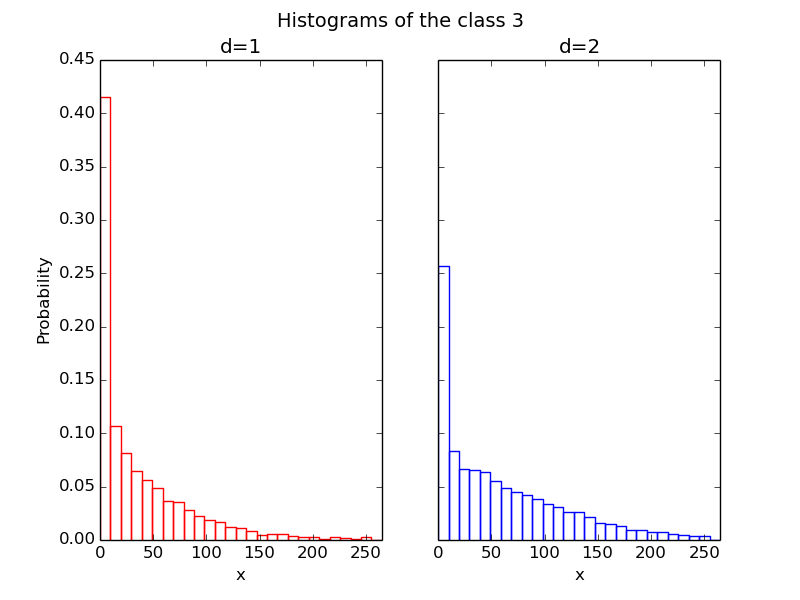
\includegraphics[width=\textwidth]{../histograms3.png}
                \caption{Class of handwritten threes}
        \end{subfigure}%
        \begin{subfigure}[b]{0.5\textwidth}
                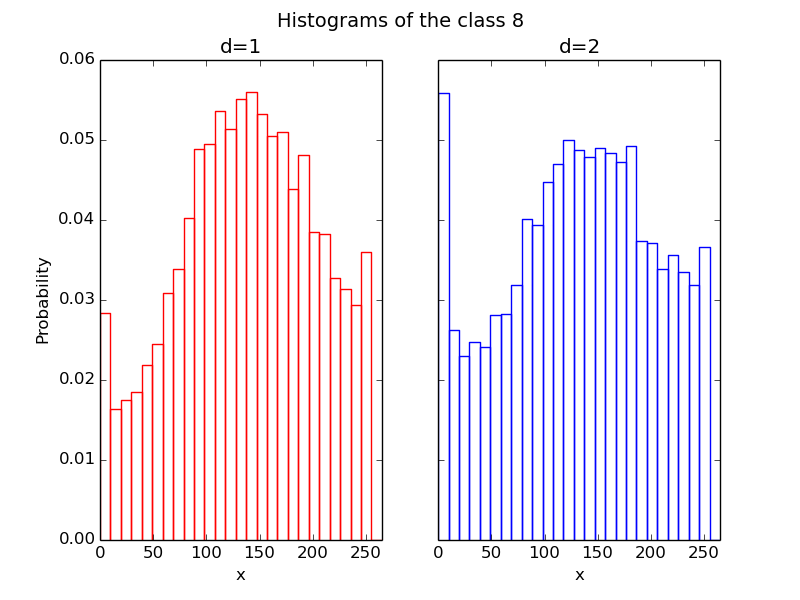
\includegraphics[width=\textwidth]{../histograms8.png}
                \caption{Class of handwritten eights}
        \end{subfigure}
        \caption{1 dimensional histograms pro class and dimension}
        \label{img1}
\end{figure}
\FloatBarrier
One the next two images we can see the visualization of the likelihoods for each class:

\begin{figure}[ht]
        \centering
        \begin{subfigure}[b]{0.5\textwidth}
                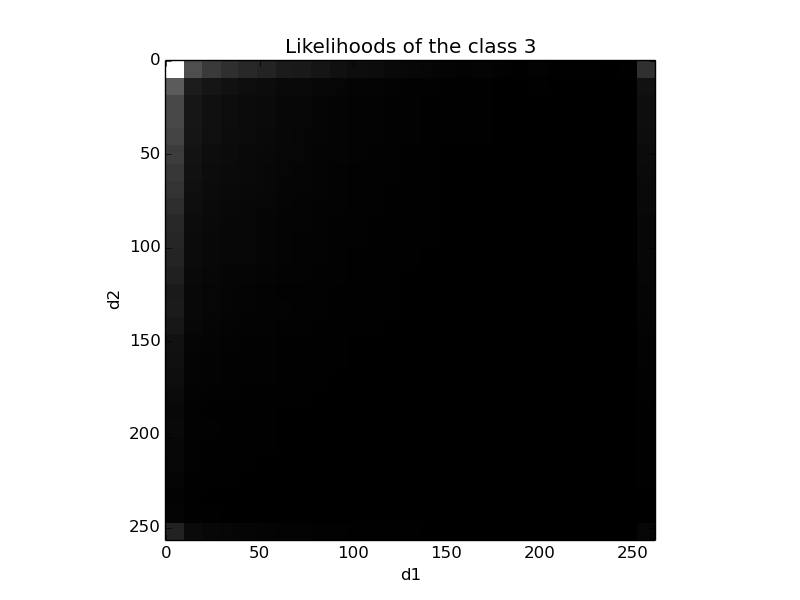
\includegraphics[width=\textwidth]{../likelihoods3.png}
                \caption{Class of handwritten threes}
        \end{subfigure}%
        \begin{subfigure}[b]{0.5\textwidth}
                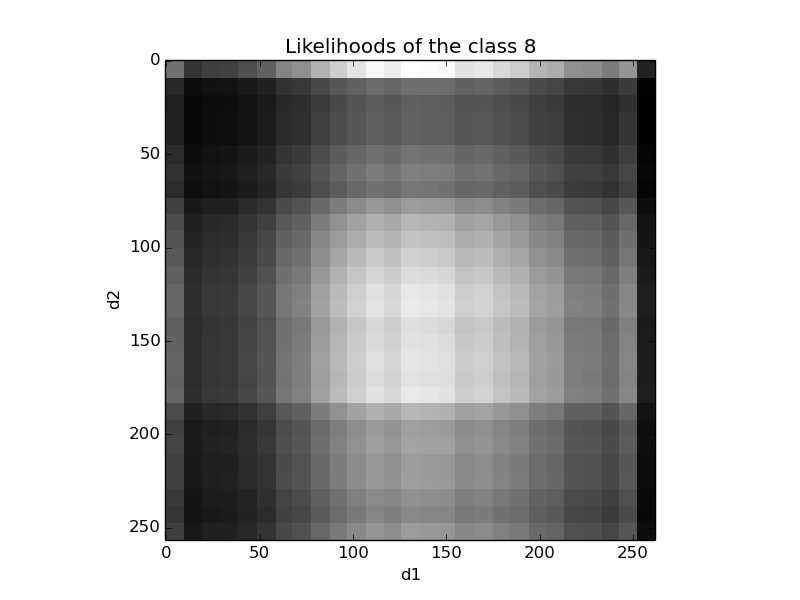
\includegraphics[width=\textwidth]{../likelihoods8.png}
                \caption{Class of handwritten eights}
        \end{subfigure}
        \caption{2D likelihoods}
        \label{img2}
\end{figure}

\FloatBarrier

After learning phase of the classifier we applied it to the images from the test set. We got the correct classification rate of $82.26\%$ (error rate = $17.74\%$) (Confusion Table see Table \ref{Table1}).

\begin{table}[hbt]
	\centering
	\begin{tabular}{|l|c|c|}
		\hline
		 & $3$ & $8$ \\ \hline
		$3$ & $9864$ & $2396$  \\ 
		$8$ & $1844$ & $9856$ \\ \hline 
	\end{tabular}
\caption{Confusion table of the naive Bayes Classifier}
\label{Table1}
\end{table}
\FloatBarrier

The classification function: 
\begin{lstlisting}[language=Python]
##                          Naive Bayes Classifier
# p3(8) priors
# p_k3(8): d rows correspond to 1D histograms pro class and dimension
def naiveBayesClassifier(testx, p3, p8, p_k3, p_k8, L, dx):
    n = testx.shape[0]
    d = testx.shape[1]
    
    prediction = np.zeros(n, dtype = np.int8)
        
    for i in range(0,n):
        x = testx[i,:]
        
        # p(y = 3| x)
        # p(y = 8| x)        
        p_y3_x = p3;
        p_y8_x = p8;
        for j in range(0,d):
            l = np.ceil(x[j]/dx[j]) # bin number         
            if l>L[j]:
                l= L[j]             
            p_y3_x *= p_k3[j][l-1]
            p_y8_x *= p_k8[j][l-1]           
        # end for j

        # argmax (p_y3_x, p_y8_x) 
        if p_y3_x>p_y8_x :
            prediction[i] = 3
        else:
            prediction[i] = 8
        # end if        
        
    # end for i
    return prediction
#end def naiveBayesClassifier
\end{lstlisting}

\subsection{Generate threes}
To construct a new digits we applied our learning algorithm to the full dimension training set ($81$ dimension) to get the likelihood for the class of threes. The sampling algorithm we used is : 
	\begin{itemize}
	\item Since we assumed, that all features are independent, we can sample in each dimension separately
	\item So for each dimension calculate from 1D histogram the cumulative distribution function (CDF); pick the uniform distributed number 	in $\alpha\in[0,1)$; calculate for each $CDF_j, j=1\dots d$, $\alpha$-quantil; return the rounded value of the $\alpha$-quantil as the $j{th}$ component of the new number.
	\end{itemize}	

Here are some results of the described generation function and the code of the function:

\begin{figure}[ht]
        \centering
        \begin{subfigure}[b]{0.5\textwidth}
                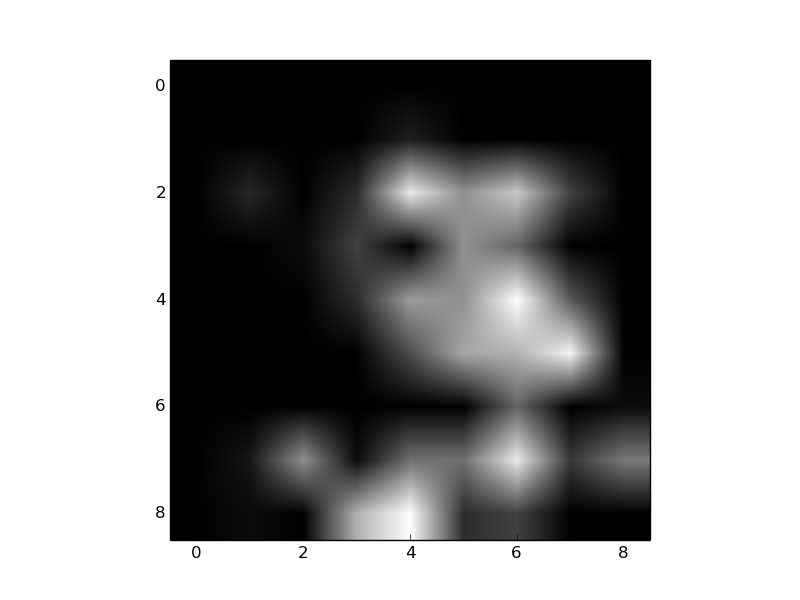
\includegraphics[width=\textwidth]{../new3nB_1.png}
        \end{subfigure}%
        \begin{subfigure}[b]{0.5\textwidth}
                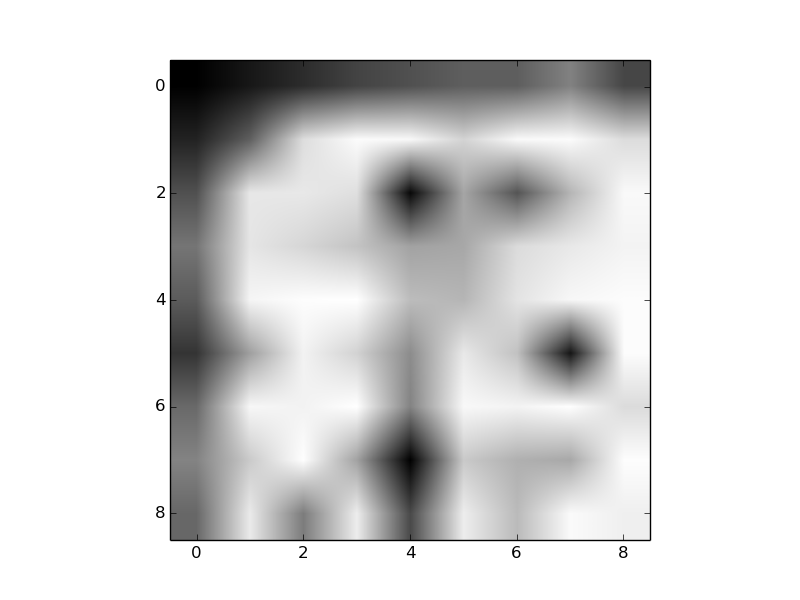
\includegraphics[width=\textwidth]{../new3nB_2.png}
        \end{subfigure}
        \begin{subfigure}[b]{0.5\textwidth}
                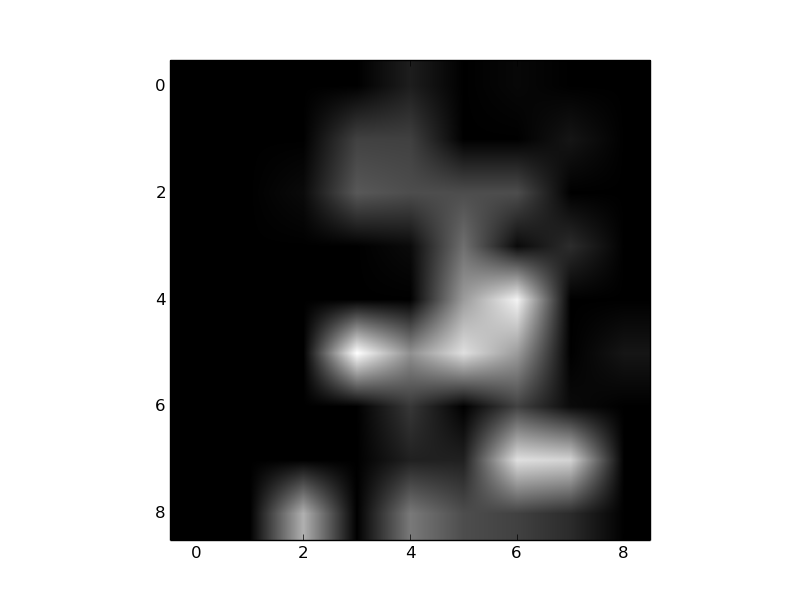
\includegraphics[width=\textwidth]{../new3nB_3.png}
        \end{subfigure}        
        \caption{Generated threes}
\end{figure}

\FloatBarrier

\begin{lstlisting}[language=Python]
## Generate Number from the given pdf
# samply in each of d dimensions independently
def generate_number(pdf,dx):
    
    d = len(pdf)    # number of dimension
    
    newnumber = np.zeros(d, dtype = np.int32)
    # calculate cumulative distribution function (cdf) from pdf
    cdf = []
    for j in range(0, d):
        cdf.append(np.cumsum(np.sort(pdf[j])) )
    # end for
        
    for j in range(0,d):
        # randomly select a uniformly distribut number in range [0., 1.)
        alpha = random.uniform(0,1)    
        # calculate quantile on the level alpha
        dist = abs(cdf[j] - alpha)
        binx = np.argsort(dist)
        
        newnumber[j] = np.floor(dx[j]*binx[0])
    # for j    
    return newnumber
# def generate_number(pdf)
\end{lstlisting}

The whole code to the naive Bayes part can be found in the file $naiveBayes.py$.

\section{Density trees}

As opposite to the naive Bayes method density tree method should keep the possible interactions between features.

\subsection{Building the DT}
We wrote a function $DT\_learning$, which starts with the single node containing all points of the training set and splits on the each iteration each node of the tree in two parts. The inputs arguments are labelled training set and splitting criteria (naive or clever).

The result of the learning are prior of the class and the list of the leaves nodes of the built density tree.

We tried out different termination criteria, such as restriction of the allowed depth or minimum density/ maximum number of points in the leaf nodes. The best results were achieved when we used the restriction with maximum number of points in leaf nodes. We also forbade splits which are two close to the region boundary. 

\begin{lstlisting}[language=Python]
#               Learning DT         
# we consider one class at time    
def DT_learning(trainingx, trainingy, c, splitmethod):
    
    print "Learning DT for the class {}". format(c)
    
    n = trainingx.shape[0]      # size of the training set
    d = trainingx.shape[1]      # size of the feature space
    
    # find  in training set all members of the class c
    xc = trainingx[trainingy==c, :]        
    nc = xc.shape[0]

    ## Priors
    prior = nc/float(n)
    
    ## Root node
    region = np.zeros((d,2), dtype = np.float32)
    for j in range(0,d):
        region[j,0] = np.min(xc[:,j])
        region[j,1] = np.max(xc[:,j])
    # end j   
      
    # build  a Density Tree and get all it's leaves  
      
    rootnode = DTnode(0, xc, 1/volume(region), region) #(depth, points, p, region)
    leaveslist = []

    stack = []
    stack.append(rootnode)
    
    while stack:
        currentnode = stack.pop()
  
        # if termination condition is satisfied (min number of points in bin):
        if currentnode.points.shape[0] < 200: 
            leaveslist.append(currentnode)
        else: # if split further
        
            if splitmethod == 'naive':
                # split value : split on the middle of two samples
                splitval, splitdim = splitnaive(currentnode) 
            else :
                # select theoretically best split
                splitval, splitdim = splitclever(currentnode, 0.5)            
            # end if clever
                 
            # new regions
            regionL = np.copy(currentnode.region)
            regionL[splitdim,:] = [regionL[splitdim,0], splitval]
            
            regionR = np.copy(currentnode.region)       
            regionR[splitdim,:] = [splitval, regionR[splitdim,1] ]           
            
            # split poins of the node according to the new regions
            pointsL, pointsR = splitpoints(currentnode.points,currentnode.region, \
                                                    splitval, splitdim)
                
            nleft = pointsL.shape[0]                  
            nright = pointsR.shape[0]                
                    
            # calculate density of the new nodes
            pL = nleft/float(nc) /volume(regionL)
            pR = nright/float(nc)/volume(regionR)        
                                   
            # create two new nodes      (depth, points, p, region)
            nodeL = DTnode(currentnode.depth + 1, pointsL, pL, regionL)
            nodeR = DTnode(currentnode.depth + 1, pointsR, pR, regionR)

            l = currentnode.region[splitdim,1]-currentnode.region[splitdim,0]   
            
            # check, if we try to split too close to region bounds
            if (splitval-currentnode.region[splitdim,0] >= 1 \
             and splitval-currentnode.region[splitdim,0] < l ):
                stack.append(nodeL) # if not add node to stack                
            else :
                leaveslist.append(nodeL) # else set node to a leaf node

            
            # check, if we try to split too close to region bounds
            if (currentnode.region[splitdim,1]-splitval >= 1 
                and currentnode.region[splitdim,1]-splitval < l ):
                stack.append(nodeR) # if not add node to stack                
            else :
                leaveslist.append(nodeR) # else set node to a leaf node

                
        # end if        
    # end while stack
    return prior,leaveslist
#end def DT_learning_naive
\end{lstlisting}

The task of the exercise was to implement two splitting methods: naive one and the theoretically best one (we called it clever splitting). 

The theoretically best criterion tries by each splitting $d(2N_c-2)$ possible split values and selects one, that maximizes the loss function (the algorithm was taken from the lecture notes). The naive splitting is a simplification of this algorithm. It tries to split in our case only at $d\times 40$ points, where $40$ points in each direction are selected as a centres of $41$ intervals of the same length along the region boundary.

Unfortunately our implementation of the theoretically best splitting is very slow, so we provide the classification results only for naive splitting method, because it is significantly faster, but we included the code for both splitting methods.

\begin{lstlisting}[language=Python]
#                            Splitting criteria
# Naive splitting method
def splitnaive(node):
    points = node.points
    d = points.shape[1]
    n = points.shape[0]
    
    nr = 40;
   
    loss = np.zeros((nr-1,d), dtype = np.float32 )
    splitvalues = np.zeros((nr-1,d), dtype = np.float32)

    for j in range(0,d):
        ind = np.argsort(points[:,j])

        dx = (points[ind[n-1],j]-points[ind[0],j])/float(nr + 1)

        for ii in range(0,nr-1):           

            splitval = points[ind[0],j] + dx*(ii+1);
            splitvalues[ii,j] = splitval
            
            # new regions
            regionL = np.copy(node.region)
            regionL[j,:] = [node.region[j,0], splitval]

            if volume(regionL)<=0.1:
                continue
                
            regionR = np.copy(node.region)       
            regionR[j,:] = [splitval, node.region[j,1] ]           

            if volume(regionR<=0.1):
                continue
                
            # split poins of the node according to the new regions
            pointsL, pointsR = splitpoints(points,node.region, \
                                                    splitval, j)
            nleft = pointsL.shape[0]
            nright = pointsR.shape[0]
                                
            loss[ii,j] = np.square(nleft /float(n))* \ 
            					(volume(node.region)/volume(regionL)) \
                       + np.square(nright/float(n))* \
                         		(volume(node.region)/volume(regionR))
        # end for i    
    #end for j
                   
    maxval = loss.max()
    valInd, dimInd  = np.where(loss==maxval)       
    splitval = splitvalues[valInd[0], dimInd[0]]    
       
    return splitval, dimInd[0]    
# end splitnaive

# select theoretically best split
def splitclever(node, eps):
    x = node.points
    d = x.shape[1]
    n = x.shape[0]
    
    loss = np.zeros((2*n,d), dtype = np.float32 )
    splitvalues = np.zeros((2*n,d), dtype = np.float32)
    for j in range(0,d):
        
        ind = np.argsort(node.points[:,j])
        for i in range(0,n):
            for s in [-1,1]:
                splitval = x[ind[2*i],j]+s*eps
                splitvalues[2*i+(s+1)/2,j] = splitval
                
                # new regions
                regionL = np.copy(node.region)
                regionL[j,:] = [regionL[j,0], splitval]
                
                if volume(regionL)<=0.1:
                    continue
                
                regionR = np.copy(node.region)       
                regionR[j,:] = [splitval, regionR[j,1] ]           
                
                if volume(regionR<=0.1):
                    continue
                
                # split poins of the node according to the new regions
                pointsL, pointsR = splitpoints(x,node.region, \
                                                    splitval, j)
                nleft = pointsL.shape[0]
                nright = pointsR.shape[0]
                    
                loss[2*i+(s+1)/2,j] = np.square(nleft/float(n))/volume(regionL) + \
                            np.square(nright/float(n))/volume(regionR)
            # end for s
        # end for i    
    #end for j                      

    maxval = loss.max()
    valInd, dimInd  = np.where(loss==maxval)       
    splitval = splitvalues[valInd[0], dimInd[0]]        
    
    return splitval, dimInd
# end splitclever
\end{lstlisting}

\subsection{Classification}

The classification task by the density trees as by naive Bayes is to calculate the probability $p(y=k|x)$ and select $k$, which maximizes this value. But in opposite to the naive Bayes method 
$$p(y=k|x)=\frac{p(x|y=k) p(y=k)}{p(x)}$$ To calculate the probability $p(x|y=k)$ we traverse all leaf nodes of the density tree to find for a given $x$ a bin, where it belongs to. In this case $p(x|y=k) = N_{bin}/{NV_{bin}}$, where $N_{bin}$ is the number of points in the found bin and $V_{bin}$ is its volume.

For the given test set we obtained the correct classification rate $79.39\%$ ( error rate $20.61\%$, for confusion table see Table \ref{Table2}). 

\begin{table}[hbt]
	\centering
	\begin{tabular}{|l|c|c|}
		\hline
		 & $3$ & $8$ \\ \hline
		$3$ & $8768$ & $3496$  \\ 
		$8$ & $1442$ & $10256$ \\ \hline 
	\end{tabular}
\caption{Confusion table of the density tree Classifier}
\label{Table2}
\end{table}
\FloatBarrier

On the picture \ref{img3} you can see the visualization of the adaptive bin of our density trees for each class. As we know from the previous section, the points of the class of threes have exponential distribution, that means we should have according to the termination criterion a lot small bins on the left top corner on the first image (see picture \ref{img3}), that are unfortunately difficult to recognize. That is why we included all images as an attachment to submitted homework.

\begin{figure}[ht]
        \centering
        \begin{subfigure}[b]{0.5\textwidth}
                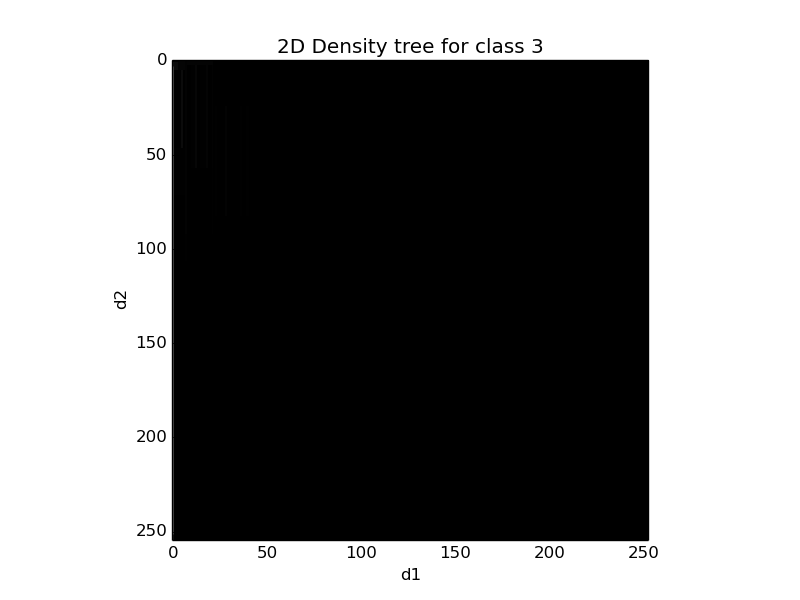
\includegraphics[width=\textwidth]{../naiveDT3.png}
                \caption{Class of handwritten threes}
        \end{subfigure}%
        \begin{subfigure}[b]{0.5\textwidth}
                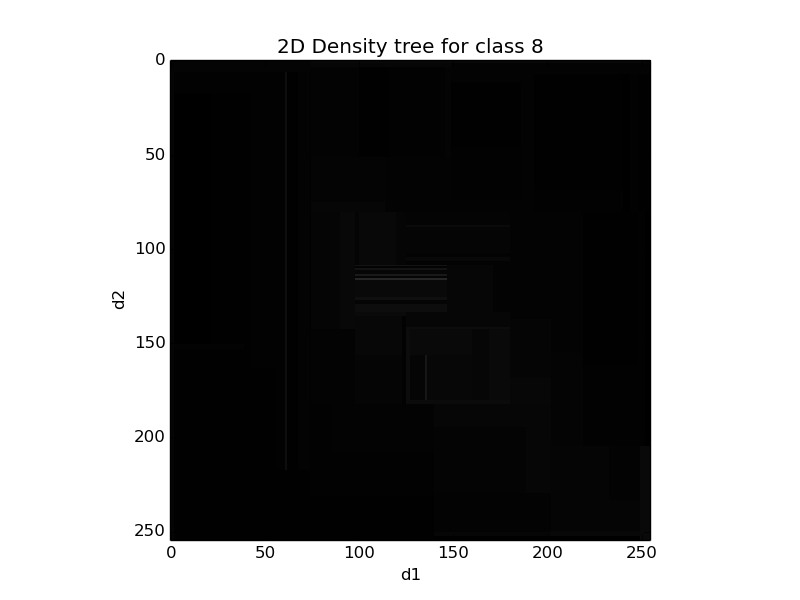
\includegraphics[width=\textwidth]{../naiveDT8.png}
                \caption{Class of handwritten eights}
        \end{subfigure}
        \caption{Adaptive bins for the density trees with naive splitting criterion}
        \label{img3}
\end{figure}


\FloatBarrier

The classification function for two classes:

\begin{lstlisting}[language=Python]
def DT_Classifier_2classes(testx, prior1, prior2, DT1, DT2, c = [3,8]):
    
    print "start classifier"
    
    n = testx.shape[0]
    
    prediction = np.zeros(n, dtype = np.int8)
    
    for i in range(0,n):
        x = testx[i,:]
            
        # p(y = 3| x)
        # find right bin in DT:
        likelihood1 = 0
        for node in DT1:
            if point_in_region(x, node.region):
                likelihood1 = node.p
                break 
            # end if
        # end for node
        p_y1_x = likelihood1*prior1
           
        # p(y = 8| x) 
        # find right bin in DT:
        likelihood2 = -1
        for node in DT2:
            if point_in_region(x, node.region):
                likelihood2 = node.p
                break 
            # end if
        # end for node        
        p_y2_x = likelihood2*prior2
           
        # argmax (p_y3_x, p_y8_x) 
        if p_y1_x>p_y2_x :
            prediction[i] = c[0]
        else:
            prediction[i] = c[1]
        # end if        
           
    # end for i    
    return prediction
# end DT_Classifier
\end{lstlisting}


\subsection{Generate threes}
For generation of new digits from the given likelihood function we implemented the following algorithm:
\begin{itemize}
\item use the whole dimensional training set to train the density tree for the digit $3$
\item start from the root node of the DT
\item with the selected probability $q$ go left in the tree and with probability $1-q$ go right; set $q=q*N_{left}/N$
\item repeat selection of the next node until a leaf node is reached
\item in the reached leaf node sample the points uniformly for each dimension
\end{itemize}

Here is the code to the described algorithm:
The traversal of the tree is done with function $DT\_traverse$, which does the same as the learning function, just doesn't return the list of leaf nodes, but a single leaf. That's why we don't call the learning function extra before.

\begin{lstlisting}[language=Python]
## Generate Number from the given pdf
# samply in each of d dimensions independently
def generate_number(trainingx, trainingy, c):
    # find  in training set all members of the class c
    xc = trainingx[trainingy==c, :]        
    d = trainingx.shape[1]      # size of the feature space
    
    ## Root node
    region = np.zeros((d,2), dtype = np.float32)
    for j in range(0,d):
        region[j,0] = np.min(xc[:,j])
        region[j,1] = np.max(xc[:,j])
    # end j   
    
    # build  a Density Tree and traverse it into depth    
    rootnode = DTnode(0, xc, 1/volume(region), region) #(depth, points, p, region)
    
    selectednode = DT_traverse(rootnode)


    # in the leaf node sample uniformly in each direction
    newnumber = np.zeros(d, dtype = np.int32) 
    for j in range(0,d):
        a = selectednode.region[j,0]
        b = selectednode.region[j,1]
        
        alpha = random.uniform(0,1)
        # transforme random number in [0,1) in random number in [a,b)
        newnumber[j] = np.floor(a + alpha*(b-a))
    # for j    
    return newnumber
# def generate_number(pdf)    
\end{lstlisting}

\begin{lstlisting}[language=Python]
# traverse the density tree: go left with probability q and right with 
# probability 1-q, generate a uniform distributed number in range [qmin, qmax)
def DT_traverse(rootnode):
    
    n = rootnode.points.shape[0]
    
    stack = []
    stack.append(rootnode)
    q = 0.5
                
    while stack:
        
        currentnode = stack.pop()
  
        # if termination condition is satisfied (min number of points in bin):
        if currentnode.points.shape[0] < 200:
            return currentnode
        else: # if split further
        
            splitval, splitdim = splitnaive(currentnode) 

            # split poins of the node according to the new regions
            pointsL, pointsR = splitpoints(currentnode.points,currentnode.region, \
                                                    splitval, splitdim)
            q = pointsL.shape[0]/float(currentnode.points.shape[0]) 
            x = random.uniform(0,1)        
            if x<=q:
                # split region
                region = np.copy(currentnode.region)
                region[splitdim,:] = [region[splitdim,0], splitval]            
                points = pointsL
            else:
                # split region
                region = np.copy(currentnode.region)       
                region[splitdim,:] = [splitval, region[splitdim,1] ]
                points = pointsR
            # end if
                
            # calculate new p
            p =  points.shape[0]/float(n) /volume(region)
        
            # go deeper
            node = DTnode(currentnode.depth+1, points, p, region)
        
            l = currentnode.region[splitdim,1]-currentnode.region[splitdim,0]   
            
            # check, if we try to split too close to region bounds
            if (splitval-currentnode.region[splitdim,0] >= 1 \
             and splitval-currentnode.region[splitdim,0] < l ):
                stack.append(node) # if not add node to stack
            else:
                return node
            # end if
        # end if        
    # end while stack
# end DT_traverse()
\end{lstlisting}        
 
 
Unfortunately, as you can seen on the next images this algorithm didn't provide good generation results.
\begin{figure}[ht]
        \centering
        \begin{subfigure}[b]{0.5\textwidth}
                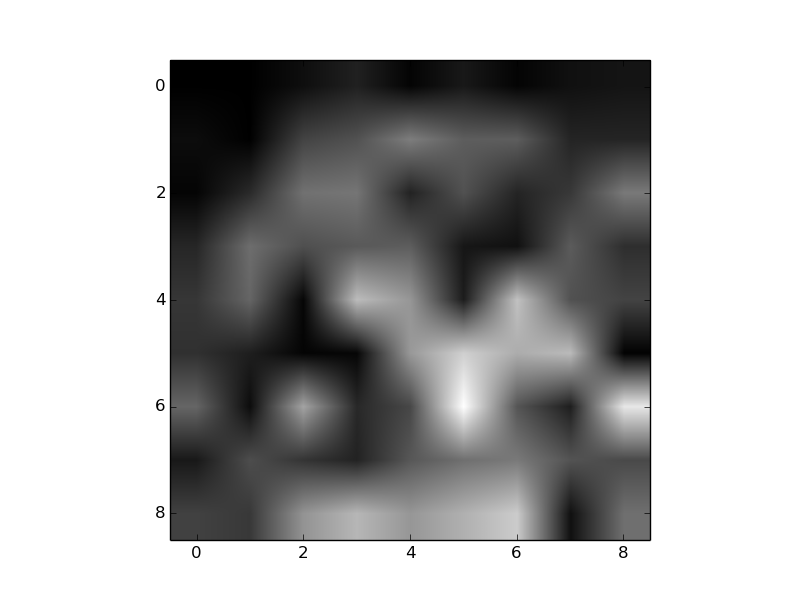
\includegraphics[width=\textwidth]{../new3DTn_1.png}
        \end{subfigure}%
        \begin{subfigure}[b]{0.5\textwidth}
                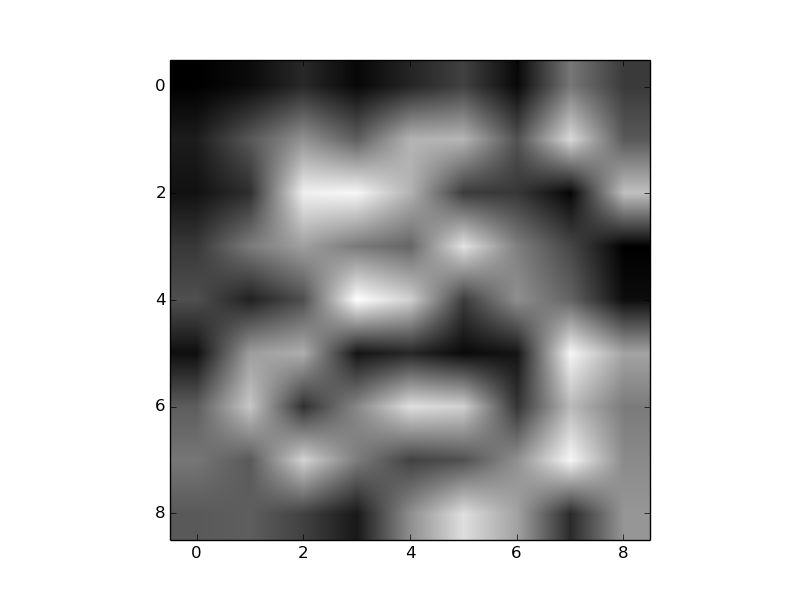
\includegraphics[width=\textwidth]{../new3DTn_2.png}
        \end{subfigure}
        \begin{subfigure}[b]{0.5\textwidth}
                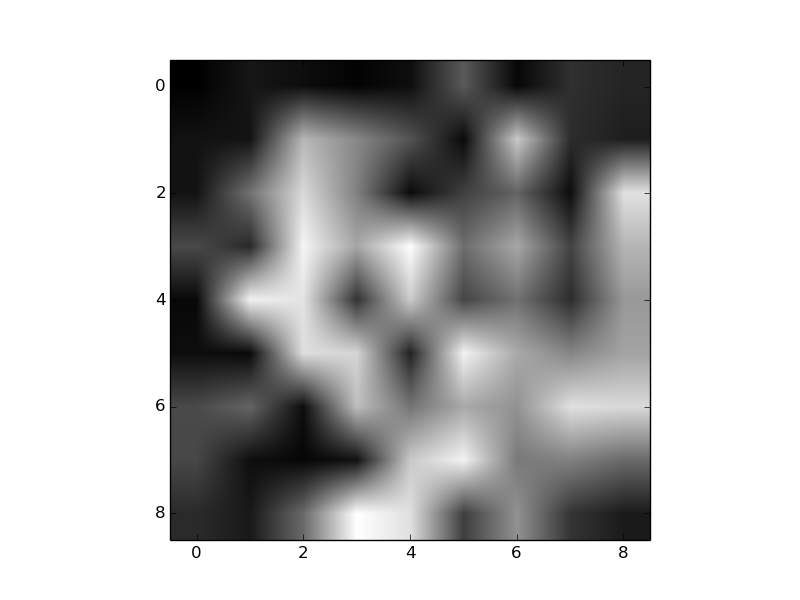
\includegraphics[width=\textwidth]{../new3DTn_3.png}
        \end{subfigure}        
        \caption{Generated threes}
\end{figure}

\FloatBarrier
All function from this section can be found in the $densityTree.py$ file in attachment.


\section{Combination of the density tree and Naive Bayes}

In the last section we want to combine naive Bayes and density trees methods. That should lead us to better modelling results.

We used the algorithms provided on the lecture to implement this part of the task

\begin{lstlisting}[language=Python]
    print    
    print "3 Combine DT and Naive Bayes"
    print
    
    n = images_train_38.shape[0]
    d = images_train_38.shape[1]

    print    
    print "Learning phase"
    print
    
    # train 1D-histogramms for each feature and class      
    
    tstart = time.time() 
    L, dx = chooseBinSize(images_train_38) # number of bins, bins size
    
    # pdf dxL matrices                  
    prior3, pdf3 = naiveBayes_train_single_class(images_train_38, \
                                                  labels_train_38, 3, L, dx)    
    prior8, pdf8 = naiveBayes_train_single_class(images_train_38, \
                                                  labels_train_38, 8, L, dx)    
    # compute the cdf of each histogramm
    cdf3 = [] 
    cdf8 = []
    pdf3sorted = []
    pdf8sorted = []
    for j in range(0, d):
        tmp = np.sort(pdf3[j])
        pdf3sorted.append(tmp)
        cdf3.append(np.cumsum(tmp) )

        tmp = np.sort(pdf8[j])
        pdf8sorted.append(tmp)        
        cdf8.append(np.cumsum(tmp) )
    # end for                                               

    tstop = time.time()
    print "Learning 1D histograms and computing cdf's took {} sec".\
                                                        format(tstop-tstart)
    
    # map data to copula using rank order transformation
    u = np.zeros(images_train_38.shape, dtype = np.float32)
    for j in range(0,d):
        ind = np.argsort(images_train_38[:,j])
        u[:,j] = ind[:]/float(n+1)
    # end for j    
    
    print
    print "Generate threes"
    
    new3th = np.zeros((3,d), dtype = np.int32)  
    for i in range(0,3) :

        u1 = generate3(u, labels_train_38 , 3 )

        for j in range(0,d):
            dist =abs(cdf3[j] - u1[j])
            binx = np.argsort(dist)
            new3th[i,j] = np.floor(dx[j]*binx[0]/2.)
        # end for j
        img = new3th[i,:].reshape(np.sqrt(d),np.sqrt(d))
        
        plot.figure()
        plot.gray()
        plot.imshow(img);
        plot.show()
     #end for i
\end{lstlisting}    

The function to generate new threes is similar to the one we used for the density trees (see file $naiveBayesAndDT.py$ for implementation):

\begin{lstlisting}[language=Python]
# traverse the density tree: go left with probability q and right with 
# probability 1-q

# Generate Number from the given pdf
# samply in each of d dimensions independently
def generate_number(trainingx, trainingy, c):
    # find  in training set all members of the class c
    xc = trainingx[trainingy==c, :]        
    d = trainingx.shape[1]      # size of the feature space
    
    ## Root node
    region = np.zeros((d,2), dtype = np.float32)
    for j in range(0,d):
        region[j,0] = np.min(xc[:,j])
        region[j,1] = np.max(xc[:,j])
    # end j   
    
    # build  a Density Tree and traverse it into depth    
    rootnode = DTnode(0, xc, 1/volume(region), region) #(depth, points, p, region)
    
    selectednode = DT_traverse(rootnode)


    # in the leaf node sample uniformly in each direction
    newnumber = np.zeros(d, dtype = np.float32) 
    for j in range(0,d):
        a = selectednode.region[j,0]
        b = selectednode.region[j,1]
        
        alpha = random.uniform(0,1)
        # transforme random number in [0,1) in random number in [a,b)
        newnumber[j] = a + alpha*(b-a)
    # for j    
    return newnumber
# def generate_number(pdf)    
\end{lstlisting}    

On the next image we provide some results of modelling for this approach:
\begin{figure}[ht]
        \centering
        \begin{subfigure}[b]{0.5\textwidth}
                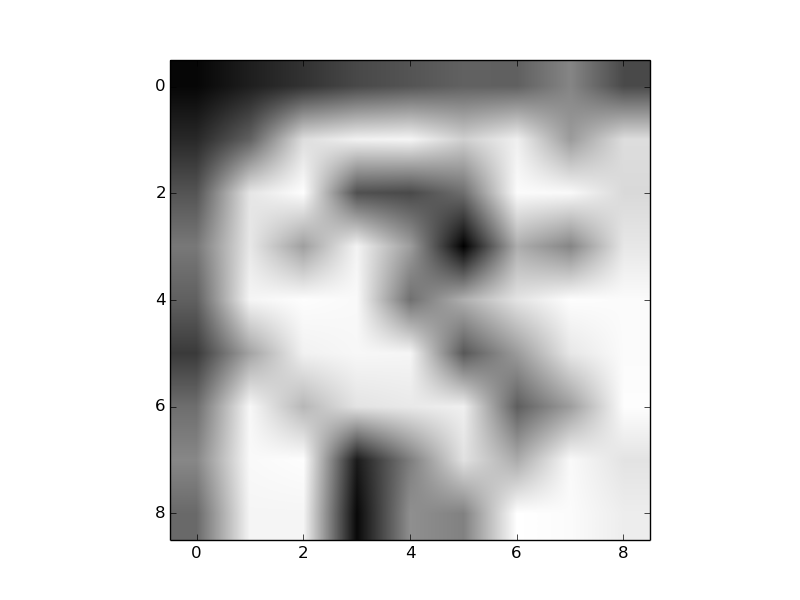
\includegraphics[width=\textwidth]{../combined_1.png}
        \end{subfigure}%
        \begin{subfigure}[b]{0.5\textwidth}
                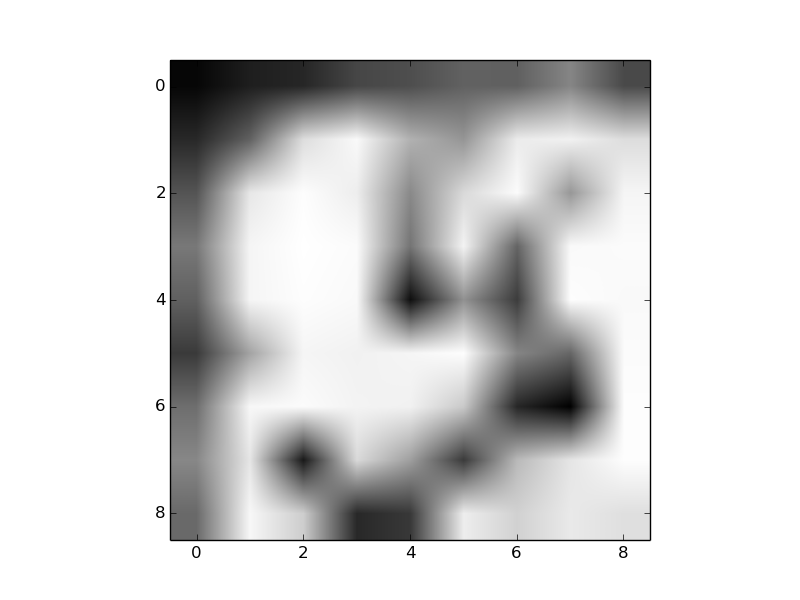
\includegraphics[width=\textwidth]{../combined_2.png}
        \end{subfigure}
        \begin{subfigure}[b]{0.5\textwidth}
                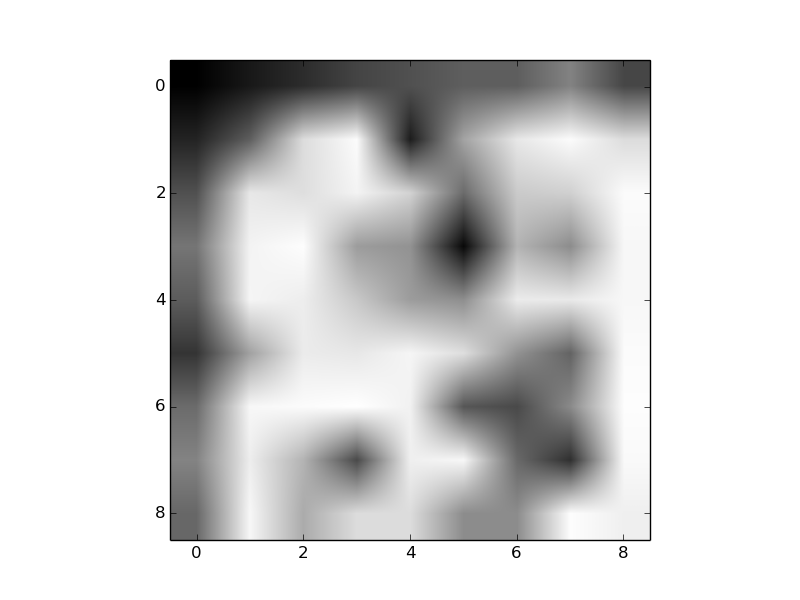
\includegraphics[width=\textwidth]{../combined_3.png}
        \end{subfigure}        
        \caption{Generated threes}
\end{figure}

\FloatBarrier

As we have supposed the results of the modelling are much better as they were before.



\section{Complete code}
\subsection{Visualization functions}

Visualization of $1D$ histograms and likelihood function for the naive Bayes method ($ex04.py$):
\begin{lstlisting}[language=Python]
#                   Plot 1D histograms
def plot_histogram(pdf,dx, title = 'Histograms for each of d dimensions',\
                                             imageName = 'histogram.png'):
    
    f, (ax1, ax2) = plot.subplots(1, 2, sharey=True)
    
    f.suptitle(title, fontsize=14)
    ax1.set_xlabel('x')
    ax1.set_ylabel('Probability') 
    
    ax2.set_xlabel('x')
    ax1.set_ylabel('Probability') 
    
    ax1.set_title('d=1')
    ax2.set_title('d=2')
    
    
    for i in range(0,len(pdf[0])):
        # subplot 1
        ax1.plot([i*dx[0], i*dx[0], (i+1)*dx[0],(i+1)*dx[0]], \
                 [0, pdf[0][i], pdf[0][i], 0 ], 'r-')
        ax1.set_xlim([0,len(pdf[0])*dx[0]])                 
    for i in range(0,len(pdf[1])):        
        # subplot 2
        ax2.plot([i*dx[1], i*dx[1], (i+1)*dx[1],(i+1)*dx[1]], \
                 [0, pdf[1][i], pdf[1][i], 0 ], 'b-')
        ax2.set_xlim([0,len(pdf[0])*dx[1]])
    # end for

    plot.show()
    
    f.savefig(imageName)    
#end def      
#-----------------------------------------------------------------------------
#                   Plot 2D Likelihood
def plot_likelihood(pdf, dx, title = 'likelihood',\
                                             imageName = 'likelihood.png'):
    L1 = len(pdf[0]) # number of bins in the first histogram
    L2 = len(pdf[1]) # number of bins in the second histogram    
    
    img = np.zeros((np.ceil(L1*dx[0]),np.ceil(L2*dx[1])), dtype = np.float64)

    for i in range(0,L1):
        for j in range(0,L2):
            img[np.ceil(i*dx[0]):np.ceil((i+1)*dx[0]),\
                np.ceil(j*dx[1]):np.ceil((j+1)*dx[1])] = pdf[0][i]*pdf[1][j]
        #end for j    
    #end for i
        
    f = plot.figure() 
    plot.gray()
    plot.imshow(img.transpose(), interpolation = 'nearest')       
    plot.title(title)
    plot.xlabel('d1')
    plot.ylabel('d2')    

    plot.show()
    
    f.savefig(imageName)    
#end def      
\end{lstlisting}    

\FloatBarrier

Visualization of the adaptive bin for the density trees ($densityTree.py$):

\begin{lstlisting}[language=Python]
def DT_visualize2D(leaveslist, trainingx, trainingy, c, saveName):

    d = trainingx.shape[1]      # size of the feature space
    
    assert d==2, 'I can visualize density trees only for two features :('
    
    # find  in training set all members of the class c
    xc = trainingx[trainingy==c, :]        
    
    d1min = np.ceil(np.min(xc[:,0]))
    d1max = np.ceil(np.max(xc[:,0]))
    
    d2min = np.ceil(np.min(xc[:,1]))
    d2max = np.ceil(np.max(xc[:,1]))
    
    img = np.zeros((d1max-d1min, d2max-d2min), dtype = np.float64)

    pmax = 0.  
    for node in leaveslist:
        if node.p>pmax:
            pmax = node.p
        xmin = np.ceil(node.region[0,0])
        xmax = np.ceil(node.region[0,1])
        
        ymin = np.ceil(node.region[1,0])
        ymax = np.ceil(node.region[1,1])

        img[xmin:xmax, ymin:ymax] = node.p
    #end for    
    
    im = np.array(img * 255/pmax, dtype = np.uint8)
    
    f = plot.figure() 
    plot.gray()
    plot.imshow(im.transpose(), interpolation = 'nearest')       
    plot.title("2D Density tree for class %d" %c)
    plot.xlabel('d1')
    plot.ylabel('d2')    

    plot.show()
   
    f.savefig(saveName)  
# end DT_visualize(DT)
\end{lstlisting}

\subsection{Naive Bayes method}
\lstinputlisting[language=Python]{../naiveBayes.py}
\subsection{Density tree method}
\lstinputlisting[language=Python]{../densityTree.py}
\subsection{Main function and Task 3}
\lstinputlisting[language=Python]{../ex04.py}

\end{document}
%------------------------------------------------------------------------------%                                    
